\documentclass[12pt]{article}
\usepackage[a4paper, hmargin={2.8cm, 2.8cm}, vmargin={2.5cm, 2.5cm}]{geometry}
\usepackage{eso-pic} % \AddToShipoutPicture

\usepackage[utf8]{inputenc}
\usepackage[T1]{fontenc}
\usepackage{lmodern}
\usepackage[english]{babel}
\usepackage{cite}
\usepackage{amssymb}
\usepackage{amsfonts}
\usepackage{amsmath}
\usepackage{enumerate}
\usepackage{mathrsfs}
\usepackage{fullpage}
\usepackage[linkcolor=red]{hyperref}
\usepackage[final]{graphicx}
\usepackage{color}
\usepackage{listings}
\renewcommand*\lstlistingname{Code Block}
\definecolor{bg}{rgb}{0.95,0.95,0.95}

%caption distinct from normal text
\usepackage[hang,small,bf]{caption}
\usepackage{hyperref}

\hypersetup{
    colorlinks,%
    citecolor=black,%
    filecolor=black,%
    linkcolor=black,%
    urlcolor=black
}

\author{
  \texttt{Gruppe: 3D} \\
  \texttt{Mikkel Enevoldsen} \\[.4cm]
  \texttt{Kristian Høi} \\[.4cm]
  \texttt{Dominique Chancelier} \\[.4cm]
  \texttt{Carsten Jensen} \\[.4cm]
  Instruktor: Jesper Lundsgaard
  \vspace{8cm}
}

\title{
  \vspace{3cm}
  \Huge{Opgave 4} \\[.25cm]
  \large{Målelige krav til brugsvenlighed}
  \vspace{.75cm}
}

\begin{document}

\AddToShipoutPicture*{\put(0,0){\includegraphics*[viewport=0 0 700 600]{includes/ku-farve}}}
\AddToShipoutPicture*{\put(0,602){\includegraphics*[viewport=0 600 700 1600]{includes/ku-farve}}}

%% Change `ku-en` to `nat-en` to use the `Faculty of Science` header
\AddToShipoutPicture*{\put(0,0){\includegraphics*{includes/ku-en}}}

\clearpage\maketitle
\thispagestyle{empty}

\newpage

%\tableofcontents %generate table of content

\thispagestyle{empty}

%\newpage
\pagestyle{plain}
\setcounter{page}{1}
\pagenumbering{arabic}

\section*{PACT}

\textbf{People}
\begin{itemize}
\item Sprogforskelle hvilke sprog synes vil v\ae re passende for FIVA
\item Hukommelse 
\item Generthed (sociale udfordringer ved henvendelse om vareplacering)
\item Socialklasser (indkomstforskelle)
\item Indkøbserfaring
\end{itemize}

\textbf{Activity}
\begin{itemize}
\item Indkøbsfrekvens  
\item Tidspres
\item Formålet veldefineret: Handle ind.
\item Præventivt varetjek. 
\end{itemize}


\textbf{Context}
\begin{itemize}
\item Supermarkeder - indkøb 
\end{itemize}

\textbf{Technology}
\begin{itemize}
\item Smartphone
\item GPS-tilgængelighed
\item Hurtighed
\item Højtlæsning af resultater
\end{itemize}

\newpage

\section*{Tjekliste til interview}
\textbf{Introduktion}\\
"Vi er datalogistuderende fra Københanvs Universitet, som skal designe en applikation omhandlende at gøre det lettere for kunden at finde varer. Vi ønsker at bruge 10 minutter på at få dine tanker omkring en sådan applikation  i et interview."
 
\begin{enumerate}
\item Fakta

\begin{enumerate}
\item Observér: Køn
\item Hvor gammel er du?
\item Hvilken teknologisk erfaring har du? Bruger du smartphone på daglig basis?
\end{enumerate}

\item Socialklasse "Hvilket erhverv og/eller uddannelsesbaggrund har du?"

\item Indkøbsfrekvens "Hvor tit handler du ind - og i hvilket tidsrum?"

\begin{enumerate}
\item Erfaring	"På hvilket niveau, erfaringsmæssigt, vil du beskrive dig selv som indkøber?"
\end{enumerate}

\item Tidsfaktor "Hvor lang tid har du til rådighed, når du handler ind?"
\item Motivation "Hvilken tilgang har du til indkøb - har du eksempelvis en struktureret plan over varer, eller køber du hvad der falder dig ind?"
\item  Vareplacering "Fortæl mig om en situation, hvor du ikke har kunnet kunne finde en vare i et supermarked."

\begin{enumerate}
\item Hjælp "Hvor ofte må du spørge en medarbejder efter hjælp?"
\item Medarbejderfravær "Hvad gør du, når du ikke kan finde en varer og ikke kan komme i kontakt med en medarbejder?"
\end{enumerate}

\item Medarb.konfrontation "Hvilke udfordringer forbinder du med at skulle opsøge en medarbejder om en vares placering?"
\item Hukommelse "Hvor mange gange om måneden glemmer du hvad du skal købe i et supermarked? - Kan du fortælle om en specifik situation?"
\item Teknologisk vane "Hvis du har en smartphone, hvordan bruger du så den i forbindelse med indkøb?"

\begin{enumerate}
\item Teknologisk til-/fravalg "Hvorfor foretrækker du smartphone frem for andre alternativer?"
\end{enumerate}

\item Præventivt varetjek "Hvordan forbereder du dig på en indkøbstur?"

\begin{enumerate}
\item "Hvis vi kigger på de sidste 100 gange du har skullet købe ind, hvor mange gange vil du skyde på at du har ringer og spurgt i forvejen om de har en vare?"
\end{enumerate}

\item Forventning "Hvad ville du forvente en sådan applikation skulle indeholde? Og hvad må den absolut ikke indeholde?"
\item Hurtighed	"Hvor lang tid vil du sige, det højst burde tage at finde en vare ved hjælp af FIVA-appen, hvorfor?"
\item Sprogforskelle "Hvilket sprog synes du FIVA-appen skal være på?"
\item Nødvendighed "Ville du bruge en varelokaliserings-app til din smartphone, hvis sådan en fandtes - hvorfor?"

\begin{enumerate}
\item Alternativer "Kan du komme på alternativer, der ville gøre en sådan applikation overflødig?"
\end{enumerate}

\end{enumerate}









\section*{Målgruppe}
\begin{itemize}
\item Kunder, der er vante smartphone-brugere, der ønsker at komme hurtigt igennem indkøb.
\item Kunder, der er vante smartphone-brugere, der handler ind til flere dage.
\item Kunder, der anvender smartphone til simpelt brug, som ønsker at komme ubesværet igennem indkøb.
\item Prisbevidste kunder der ønsker billigere varer.
\end{itemize}

\subsection*{Målgruppebeskrivelse}
Målgruppen handler ind 3-4 gange om ugen. De ønsker en let og hurtig indkøbstur, hvor eventuelle problemer hurtigt ville kunne løses gennem FIVA-appen. De ønsker problemfrit at finde varer, som de sjældent køber.\\
Brugerne er vante indkøbere, og kender derfor det forventede varesortiment i butikken de ønsker at handle i.\\

\noindent Målgruppen bruger deres smartphones generelt til normal kommunikation, så som at ringe, sms og internetsøgninger. Brugeren ved hvad applikationer er, og bruger forbrugsapps, som eksempelvis Danske Banks mobilbank, Google Maps og Rejseplanen efter behov.\\

\noindent Målgruppen forstår at bruge en søgefunktion og følge en GPS' angivelser. De ved ikke hvordan smartphonen og appen fungerer internt. For dem er en smartphone, et redskab til at gøre hverdagen lettere.

\section*{Personas}

\subsection*{Lars Jensen}

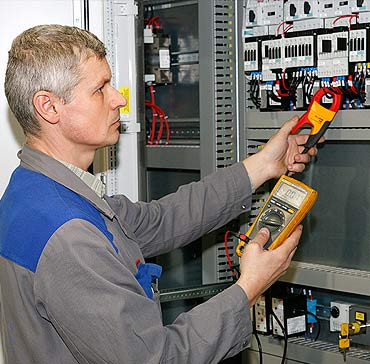
\includegraphics[scale=0.5]{includes/lars.jpg}

Lars Jensen er 57 år og bor i en forstad til Aarhus. Her han boet han sammen med sin kone, Lis Jensen, i de sidste 25 år. Sammen har de to børn, Michael på 18 og Anne på 21, der begge er flyttet hjemmefra.\\

\noindent Lars er uddannet elektriker, og har været vant til at gøre tingene selv i det meste af sit liv. Lars har haft en smartphone i omkring 2 år, og er ved at blive fortrolig med dens smarte funktioner.\\

\noindent Når der skal handles ind, er det oftest konen der sørger for det. Men desværre er Lis' hukommelse ikke hvad den har været, så derfor må Lars af og til ned og købe de enkelte ting hun glemmer. Han synes det er irriterende, at han så ofte må spørge medarbejdere om hjælp til at finde de forskellige varer. Han synes det spilder tiden for begge parter.


\subsection*{Maria Møller}

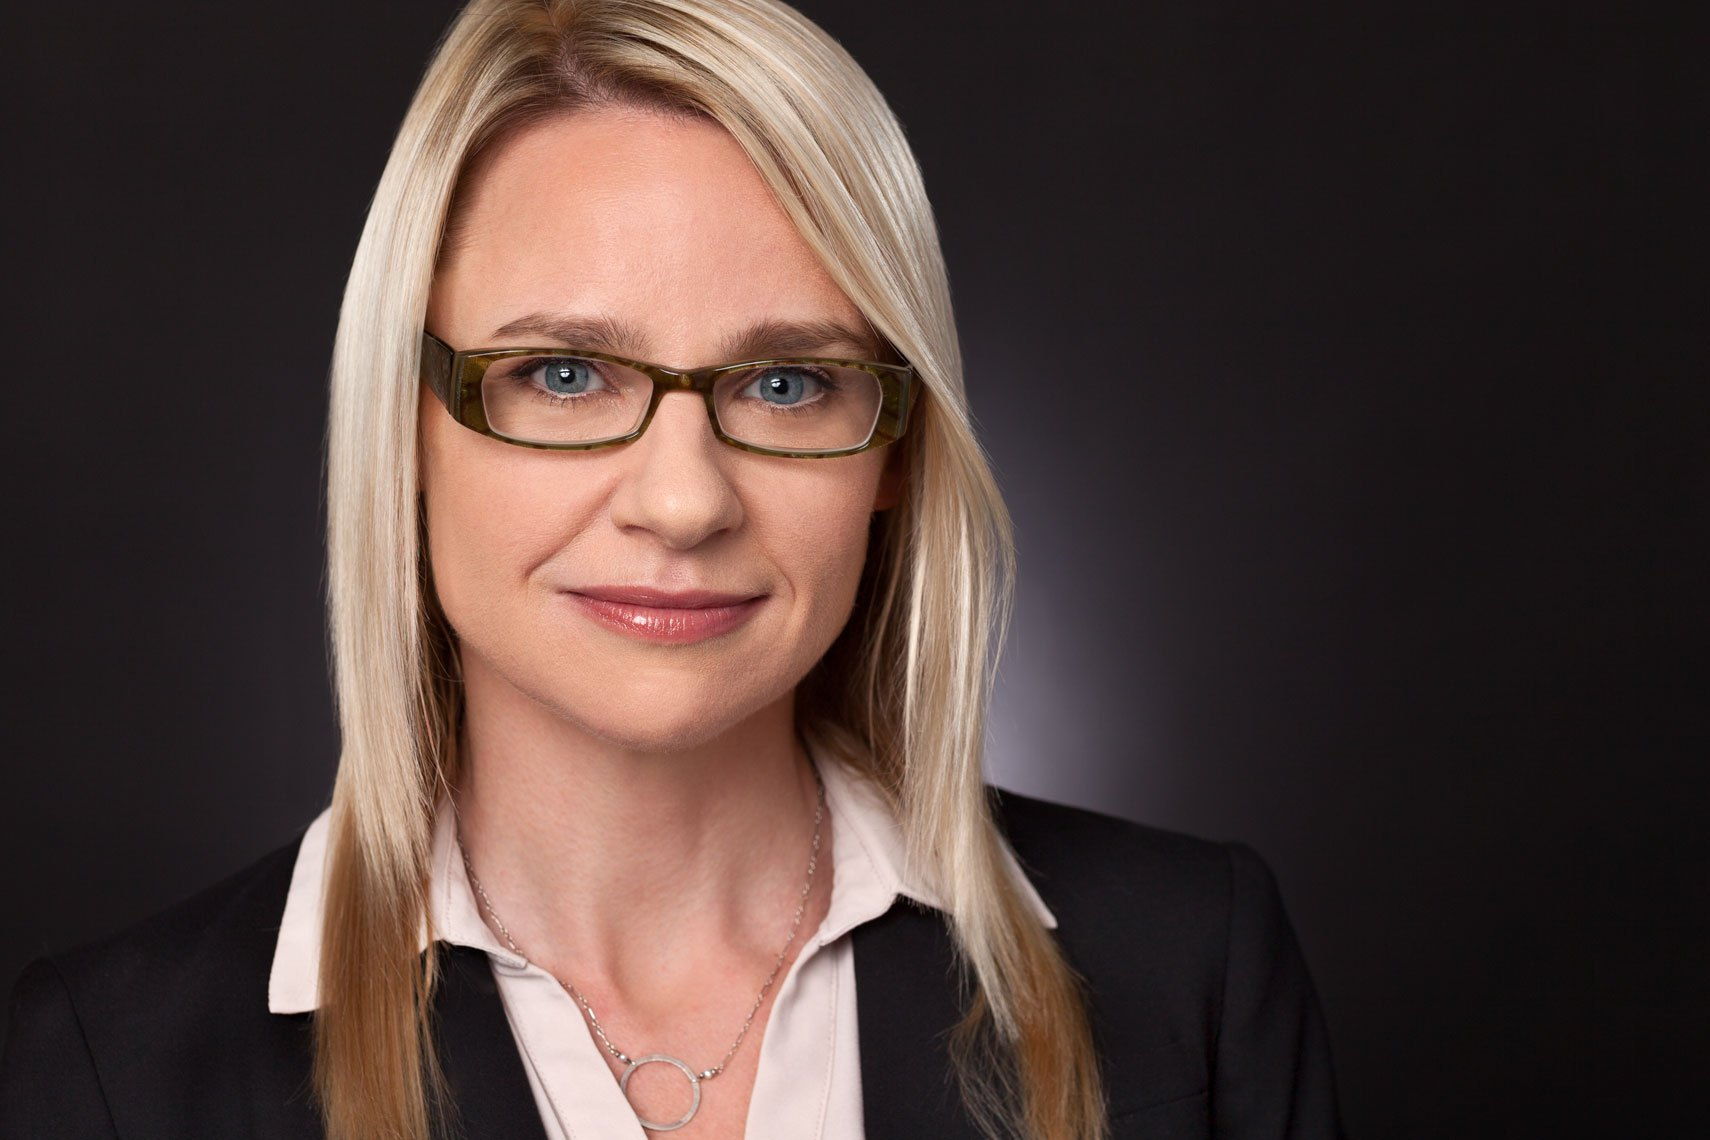
\includegraphics[scale=0.2]{includes/maria.jpg}

\noindent Maria Møller er 36 år og bor på Vesterbro i København. Hun bor sammen med sin søn, Emil, på 4 år. Maria er uddannet journalist på RUC, og er ansat på dagbladet Information. Hun har haft en smartphone i omkring 7 år og bruger den dagligt til at kommunikere med familie og venner samt tjekke nyheder.\\

\noindent Maria er glad for at udforske forskellige madkulturer, og hendes yndlingskøkkener er det asiatiske eller mexicanske. Dog har hun for nyligt begyndt at blive inspireret af det nynordiske køkken. Derfor handler hun mange forskellige og nye varer, som hun ikke altid ved hvor er i butikken. Derfor må hun ofte spørge medarbejderne om hjælp - og har oplevet flere gange, at de heller ikke ved hvor varen er.

\section*{Scenarier}
\subsection*{Lars Jensen}
Lars får at vide, at han skal ned og købe fennikel og kaffefiltre. Når Lars ankommer til supermarkedet åbner han sin nye FIVA-app og indtaster fennikel og kaffefilter i søgefunktionen. Lars har nu en rute, som han følger og finder sine varer. Han bruger "Gå til kassen"-funktionen, og får sin rute til kassen. Lars betaler, og skynder sig hjem.

\subsection*{Maria Møller}
Maria sidder derhjemme og planlægger sin indkøbsliste. Her bruger FIVA-appen til at indskrive alle sine varer. Når Maria senere på dagen går ned for at handle, åbner hun appen og beder om ruten til sin indkøbsliste. Hun følger sin rute, men kommer undervejs i tanke om at hun også skal have artiskokker, som hun tilfældigvis ikke ved hvor ligger. Hun taster ind i appen, som tilpasser til hendes rute og viser placeringen på artiskokker. Hun finder sine artiskokker, og fortsætter sin rute.





\end{document}
